%------------------------------------ Inicio ---------------------------------------
\documentclass[11pt, a4paper]{article}

% -------------- Nombre del documento --------------
\newcommand{\nombre}{Trabajo Practico N°2}
%---------------------------------------------------------

%-------------------- Include Paquetes iniciales---------------------
\usepackage{mathtools}
\usepackage{graphicx}
\usepackage{float} 
\usepackage{geometry}
\usepackage{setspace}
\geometry{top=35mm,bottom=30mm,left=33mm,right=33mm,headsep=15mm}
\usepackage{relsize} % agranda a un mas las letras
\usepackage[spanish,es-nodecimaldot]{babel}
\usepackage[utf8]{inputenc}
\usepackage{lastpage} % nos dice el numero total de paginas
\usepackage{fancyhdr} % modifica encabezado y pie de pagina
\pagestyle{fancy} % Con ésto aplicamos el encabezado y pie 
\renewcommand{\headrulewidth}{0.2pt} % linea encabezado tamaño
\renewcommand{\footrulewidth}{0pt} % linea pie de pagina tamaño

\cfoot{}
\pagestyle{fancy}
\fancyhf{}
\rfoot{\thepage}
\lhead{
\includegraphics[scale=0.12]{Imagenes/logounc.jpg}}
\rhead{\nombre}
%-----------------------------------------------------------------------


\begin{document}

%--------------------  Portada ---------------------


\begin{center}
	{\huge\textbf{SINTESIS DE REDES}} \\
	\vspace{3mm}
	{\huge\textbf{ACTIVAS}} \\
	\vspace{10mm}
	{\large -}
	\vspace{2mm}
	
\begin{figure}[H]
	\centering
	
\includegraphics[width=0.7\linewidth]{Imagenes/logoPrincipal.png}
\end{figure}
\vspace{10mm}
\textscale{3}{ \textbf{\nombre}} \\
\vspace{8mm}
\textscale{1.6}{ AO REAL: Errores\textbf{}}\\
\vspace{6mm}
	\textscale{1.3}{ Síntesis de Redes Activas - 2024\textbf{}}\\
	\vspace{15mm}
	---------------------------------------------\-\\
	\vspace{15mm}
	\textscale{1.3}{\textbf{Integrantes}}\\
	\vspace{6mm}
	\textscale{1.3}{Valentin Jose Ramirez, 43700362}\\
 \vspace{2mm}
	\textscale{1.3}{José Ignacio Lopez Sivilat, 44805902}\\
 \vspace{2mm}
	\textscale{1.3}{Franco Gabriel Lopez, 43271762} \\
     \vspace{2mm}
	\textscale{1.3}{Alejo Adrian Beierbach, 43700333} \\
	\vspace{15mm}
	\textscale{1.3}{\textbf{Profesores adjuntos}}\\
 \vspace{6mm}
 \textscale{1.3}{Dr. Ing. Pablo A. Ferreyra}\\
 \vspace{2mm}
 \textscale{1.3}{Ing. César Reale}\\
	\thispagestyle{empty}
\end{center}
\clearpage
%----------------------------fin portada-----------
\thispagestyle{empty}
\tableofcontents
\clearpage


% ------------------------------------- Desarrollo ---------------------------------
\pagenumbering{arabic}

\newpage
\section{Consigna}
\paragraph{}
\subsection{Objetivos}
Introducir al estudiante en el diseño, armado, medición y análisis de circuitos amplificadores lineales, teniendo en cuenta las fuentes de error del AO real, y como se relacionan con
las condiciones de entorno del circuito.
En este trabajo de laboratorio se lleva a cabo el análisis de funcionamiento del un amplificador real para lo cual se tiene en cuenta las fuentes de error presentes en el mismo, causantes de que la salida final presente una desviación respecto a la respuesta ideal teórica. El circuito sobre el cual se lleva a cabo el estudio es un sumador inversor. 
\paragraph{}
Los errores sobre los cuales se realiza el análisis son:
\begin{itemize}
    \item \textbf{Errores en DC:}
    \begin{enumerate}
	\item Error de tensión, $v_{os}$.
	\item Error de corriente, $I_{os}$.
	\item Error por $A_d<\infty$.
        \item Error por $RRMC<\infty$.
    \end{enumerate}
    \item \textbf{Errores en AC:}
    \begin{enumerate}
        \item Error vectorial.
        \item Ancho de banda a plena potencia.
        \item Ancho de banda para pequeña señal.
    \end{enumerate}
\end{itemize}
\paragraph{}
Para cada circuito, se realizará un análisis teórico, simulaciones y mediciones experimentales. Finalmente, se van a comparar los datos obtenidos en cada etapa.
\newpage
\section{Circuito I: Sumador Inversor}
\begin{figure}[htb]
	\centering
	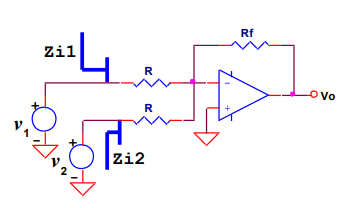
\includegraphics[width=1\textwidth]{Imagenes/Circuito1.png}
	\caption{Circuito propuesto}
\end{figure}
\subsection{Requisitos}
Para el desarrollo del presente trabajo se empleará un circuito sumador inversor utilizando el amplificador operacional \textit{LM324}. El circuito debe cumplir con las siguientes especificaciones:
\begin{itemize}
    \item $V_{cc}=10[V]$ y $V_{ss}=-10[V]$
    \item $A_{v|v_1}=30$, $A_{v|v_2}=30$
    \item $R_i<<Z_{i1}$, $R_i<<Z_{i2}$
    \item Emplear resistencias menores a $10[M\Omega]$
\end{itemize}

\newpage

\section{Análisis teórico}
A continuación se obtienen las ecuaciones pertinentes para el cálculo de errores.

\subsection{Ganancia ideal en banda de paso}
\onehalfspacing
\begin{flushleft}
    \textbf{Pasivando $V_2$}\\
    $V_{O}|_{V_2=0}=-\frac{R_f}{R}$ \\
    \textbf{Pasivando $V_{1}$} \\
    $V_{O}|_{V_{1}=0}=-\frac{R_f}{R}$ \\
\end{flushleft}
\begin{center}
    \boxed{V_{O}=A_1\cdot v_1 + A_2 \cdot v_2}\\
    reemplazando con $A_1=A_2=-\frac{R_f}{R}$ \\
    \boxed{V_{O}=-\frac{R_f}{R}\cdot (v_1+v_2)}
\end{center}

\subsection{Errores en DC}
\onehalfspacing
Del circuito general, pasivando las entradas, se calcula la ganancia de lazo.
\begin{center}
    \boxed{T(S)=-\frac{R}{R+2R_f}\cdot A_d(S)}
\end{center}
Para obtener las ecuaciones que describen cada error se emplea la ecuación de $Blackman$ y se suponen el resto de las característiscas del amplificador ideal a excepción de la de interés.

\subsubsection{Error por tensión de offset, $v_{os}$}
\onehalfspacing
El error por tensión de offset se estima colocando en la entrada no inversora una fuente de tensión constinua de valor $v_{os}$
\begin{center}
    \boxed{\frac{V_{O}}{V_{os}} = 1 + \frac{R_f}{R_p}}\\
    donde $R_p=\frac{R}{2}$; reemplazando \\
    \boxed{V_{O} = (1 + 2\cdot\frac{R_f}{R}) \cdot v_{os}}
\end{center}

\subsubsection{Error por corrientes de bias, $I_{os}$}
\onehalfspacing
Debido a que no hay una resistencia asociada a la entrada no inversora la corriente $I^{+}_p$ no produce error, en consecuencia el error en la salida solo está definido por $I^{-}_p$
\begin{center}
    \boxed{\frac{V_O}{V^{-}}=\frac{R+2R_f}{R}}
\end{center}
Donde $V^{-}=I^{-}_p\cdot R_p$, $R_p=\frac{R_f\cdot R}{2R_f+R}$, por lo que resulta,
\begin{center}
    \boxed{V_O(I_p^{-})=-I_p\cdot R_f}
\end{center}

\subsubsection{Error por $A_d<\infty$}
\onehalfspacing
La ganancia real de un amplificador puede definirse como:
\begin{center}
    \boxed{A_v(s)=\frac{A_{vfi}}{1-\frac{1}{T(s)}}}
\end{center}
Donde:
\begin{itemize}
    \item $A_{vfi}:$ ganancia ideal para la configuración seleccionada.
    \item $T(s):$ ganancia de lazo.
\end{itemize}
\paragraph{}
Si $A_d(s)\rightarrow \infty$ entonces $T(s) \rightarrow \infty$ por lo que el error para $A_d(s)<\infty$ como:
\begin{center}
    \boxed{\epsilon_{G0}=\frac{1}{T_O}}
\end{center}
\paragraph{}
Luego,
\begin{align}
    \nonumber
    A_{vf}(s) &= \frac{A_{vfi}}{1 + \epsilon_G(s)} \\
    \nonumber
    A_{vf}(0) &= \frac{A_{vfi}}{1 + \epsilon_G(0)} \\
    \nonumber
    A_{vf}(0) &= A_{vfi}(1-\epsilon_G(0))
\end{align}
\paragraph{}
Despejando $\epsilon_G(0)$ y reordenando,
\begin{center}
    \boxed{\Delta V_0 = \epsilon_G(0)\cdot V_{0i}}
\end{center}
\paragraph{}
De la ecuación anterior se tiene que el máximo error sucede cuando $V_{0i}=FS$,
\begin{center}
    \boxed{\Delta V_{0, max}(A_d<\infty)=\epsilon_G(0)\cdot FS=\frac{FS}{T_O}}
\end{center}

\subsubsection{Error por $RRMC<\infty$}
\onehalfspacing
Debido a que la entrada no inversora está conectada a masa el error producido por $RRMC<\infty$ resulta despreciable ya que la tensión común es mínima.

\newpage

\subsection{Errores en AC}
\onehalfspacing
Para el análsis en AC se debe contemplar la expresión que define el comportamiento de la ganancia del amplificador en función de la frecuencia.
\begin{center}
    \boxed{A_{vf}(s)=\frac{A_{vf}(0)}{(1+\frac{s}{\omega_H})}}
\end{center}

\subsubsection{Ancho de banda a plena potencia}
\onehalfspacing
Se define como la máxima frecuencia que puede presentar la señal de entrada para ser reproducida en la salida sin distorsión,
\begin{center}
    \boxed{\omega_{HP}=\frac{SR}{V_{pp}}}
\end{center}
de donde,
\begin{itemize}
    \item $SR:$ Slew-Rate.
    \item $V_{pp}:$ Tensión pico a pico máxima.
\end{itemize}

\subsubsection{Ancho de banda de pequeña señal}
\onehalfspacing
Se define así al punto donde la ganancia cae $-3dB$ respesto al valor en la banda de paso. Del producto $GBW$ se obtiene,
\begin{equation}
   \nonumber
   \omega_H \cdot A_{vf} = \omega_T 
\end{equation}
\begin{center}
    \boxed{\omega_H = \frac{\omega_T}{A_{vf}}}
\end{center}

\subsubsection{Error vectorial}
\onehalfspacing
Se define como la diferencia entre la ganancia ideal y la real:
\begin{center}
    \boxed{E_v=A_{vfi}-A_{vf}(s)}
\end{center}
Dado que le resultado lo conforma un vector se puede dividir en \textit{error de ganancia} y \textit{error de fase}.
\paragraph{}
\textbf{Error de ganancia}
\onehalfspacing
Se define de esta manera a la diferencia entre los módulos real e ideal. Normalizando la ecuación para el error vectorial en función de $A_{vfi}$:
\begin{align}
    \nonumber
    e_v&=|1| - \abs{\frac{1}{1+\frac{s}{\omega_H}}} \\
    \nonumber
    e_v &= 1 - \frac{1}{\sqrt{1+\frac{\omega}{\omega_H}^2}}
\end{align}
Se puede aproximar a:
\begin{center}
    \boxed{e_v = 1 - \sqrt{1+\frac{\omega}{\omega_H}^2}}
\end{center}

\paragraph{}
\textbf{Error de fase}
\onehalfspacing
Es la diferencia entre las fases de la ganancia ideal y la ganancia real:
\begin{center}
    \boxed{\Phi_v = -\arctan{(\frac{\omega}{\omega_H})}+\frac{\pi}{2}}
\end{center}
\newpage

\section{Caso de estudio para $R_i=50[\Omega]$}

\subsection{Diseño de la etapa.}
\onehalfspacing
Entre los requisitos de diseño mencionados se solicita que la impedancia de entrada no cargue a la fuente, que se trabaje con resistencias menores a $1[M\Omega]$ y que la ganancia para cada fuente sea de $30$ veces.
\paragraph{}
A partir de dichas especificaciones se obtiene:
\begin{equation}
    \nonumber
    R_i=50[\Omega] \longrightarrow Z_{i1,2} \geq 10R_i
\end{equation}
donde $Z_{i1,2} = R$.
\paragraph{}
Tomando $R=1[k\Omega]$ y recordando que $A_{v1,2}(0)=30$
\begin{equation}
    \nonumber
    \frac{R_f}{R}=30 \longrightarrow R_f=30[k\Omega]
\end{equation}

\subsection{Cálculo de errores.}
\onehalfspacing
A partir de las características eléctricas del $LM324$ se calculan los respectivos errores.

\subsubsection{Errores en DC.}
\onehalfspacing
\begin{equation}
    \nonumber
    \Delta V_{O}(v_{os}) = \left(1+2\frac{R_f}{R}\right) \cdot v_{os} = 61v_{os} = 61\cdot 2[mV]  = 122[mV]
\end{equation}
\begin{equation}
    \nonumber
    \Delta V_{O}(I_{os}) = -R_f\cdot I_p^{-} = 30[k\Omega]\cdot I_p^{-} = 30[k\Omega]\cdot 45[\mu A]  = 1350[\mu V]
\end{equation}
\begin{equation}
    \nonumber
    \Delta V_{O}(A_d<\infty) = \frac{FS}{T_O} = \frac{10[V]}{1640} = 6.1[mV]
\end{equation}
\begin{equation}
    \nonumber
    \Delta V_{O}(RRMC<\infty) = 0[V]
\end{equation}

\subsubsection{Errores en AC.}
\onehalfspacing
\textbf{Ancho de banda de plena potencia.} 
\paragraph{}
\begin{equation}
    \nonumber
    f_{HP} = \frac{SR}{2\pi \cdot V_{pp}} =  \frac{0.5\left[ \frac{V}{uS} \right]}{2\pi \cdot 10[V]} = 8[kHz]
\end{equation}

\paragraph{}
\textbf{Ancho de banda de pequeña señal.} 
\paragraph{}
\begin{equation}
    \nonumber
    f_{HP} = k\cdot f_T = \frac{R}{R+2R_f}\cdot f_T = 16.4[kHz]
\end{equation}

\paragraph{}
\textbf{Error vectorial.} 
\paragraph{}
\begin{figure}[h!]
    \centering
    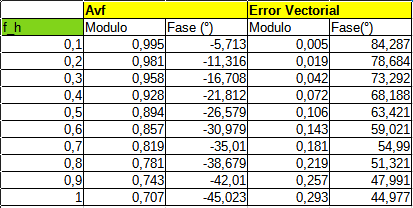
\includegraphics{Imagenes/tabla1.png}
    \caption{Error vectorial}
    \label{fig:enter-label}
\end{figure}


%\newpage

\subsection{Simulaciones.}
\onehalfspacing
Realizamos las mediciones del primer caso para el siguiente circuito simulado en LTSpice:
\begin{figure}[h!]
    \centering
    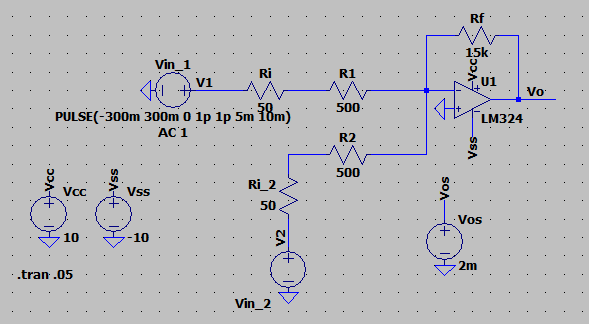
\includegraphics[scale=0.8]{Imagenes/CircSim2.png}
    \caption{Circuito simulado}
    \label{fig:enter-label}
\end{figure}

\begin{figure}[h]
    \centering
    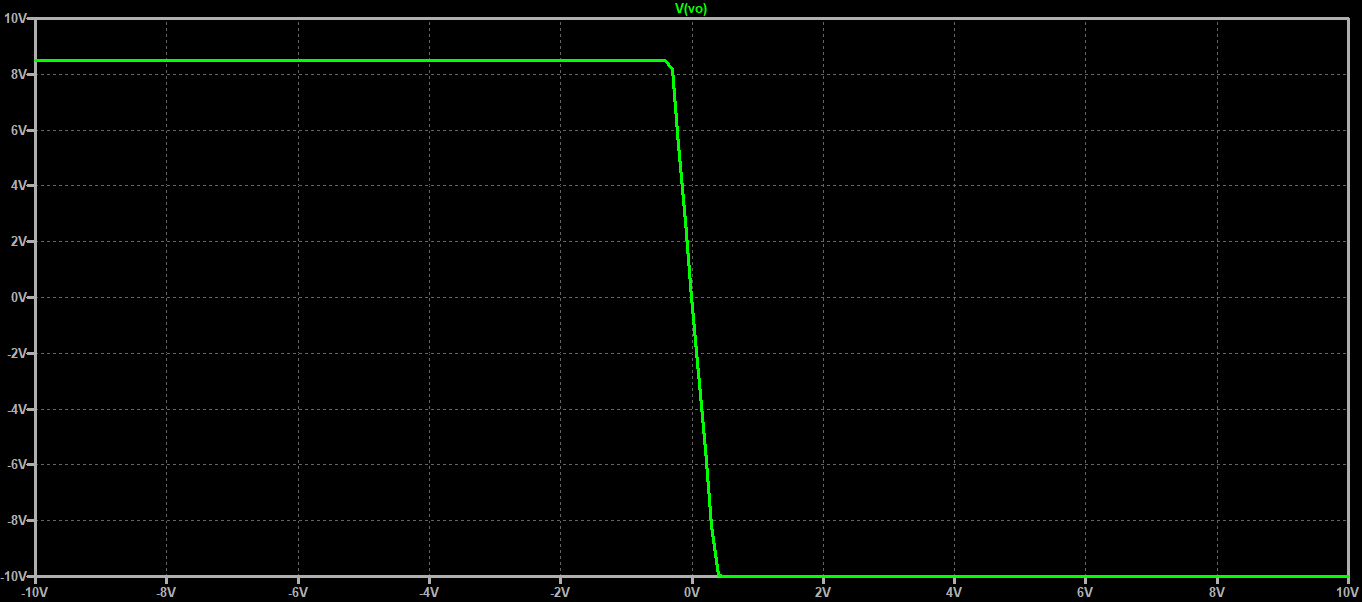
\includegraphics[scale=0.4]{Imagenes/barrido_-10V_10V_continua.png}
    \caption{Barrido en frecuencia}
    \label{fig:enter-label}
\end{figure}

\begin{figure}[H]
    \centering
    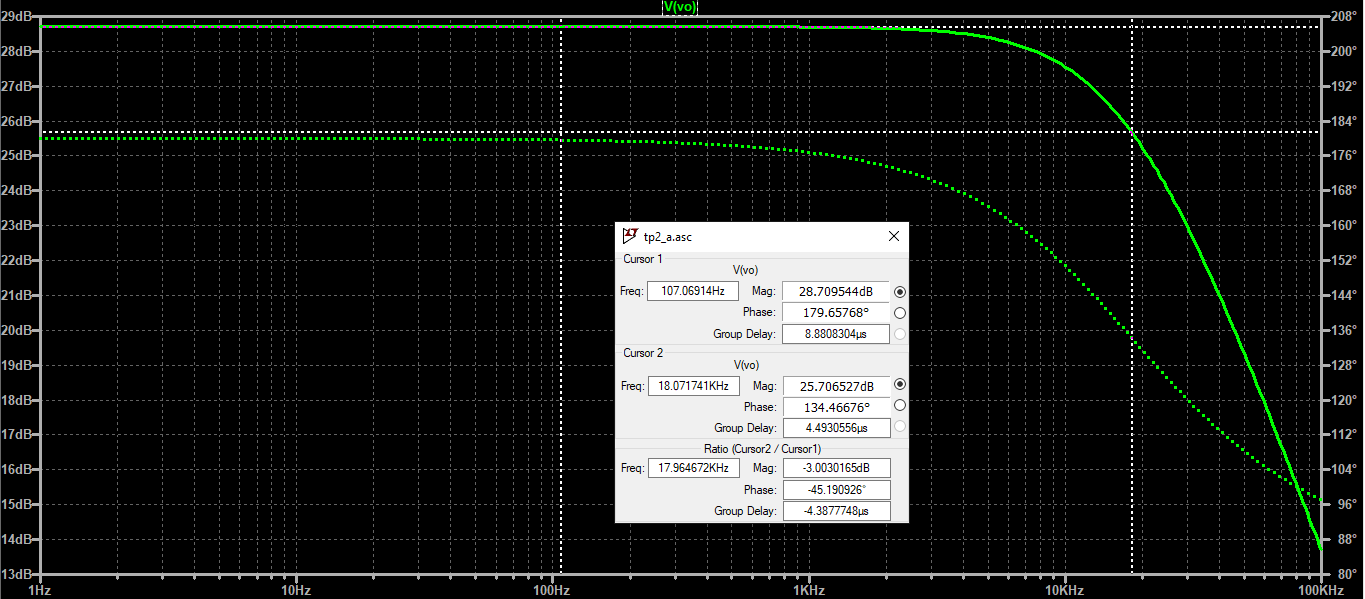
\includegraphics[scale=0.4]{Imagenes/bode.png}
    \caption{Diagrama de Bode}
    \label{fig:enter-label}
\end{figure}
\begin{figure}[H]
    \centering
    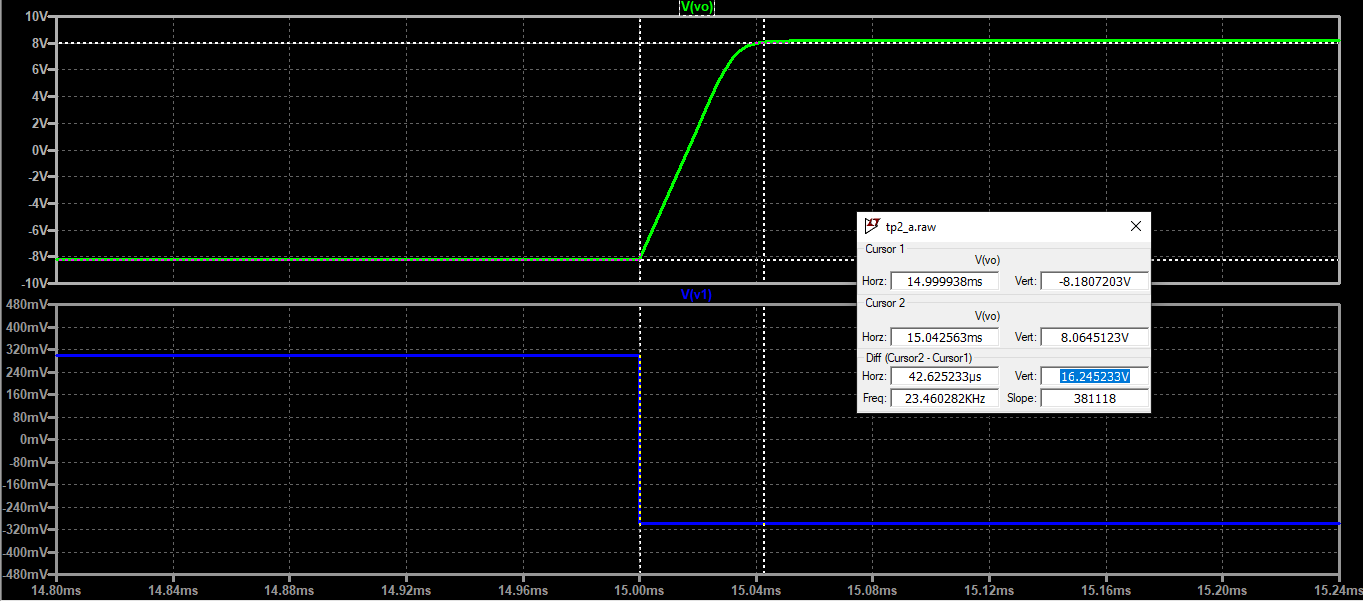
\includegraphics[scale=0.4]{Imagenes/Slew_Rate_Vin=600mV_PP.png}
    \caption{Slew Rate}
    \label{fig:enter-label}
\end{figure}
\begin{figure}[H]
    \centering
    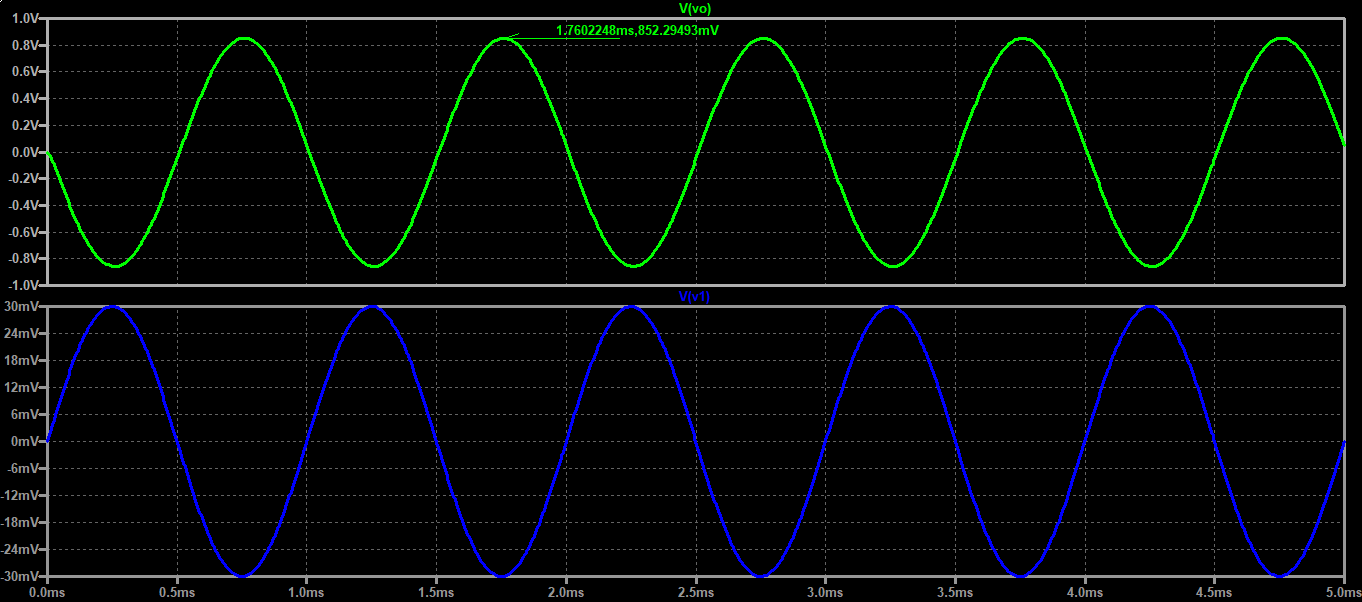
\includegraphics[scale=0.4]{Imagenes/Vo_Vin=30mV_CA_Ri=50.png}
    \caption{Factor de amplificación, $A_v = 30$}
    \label{fig:enter-label}
\end{figure}
\begin{figure}[H]
    \centering
    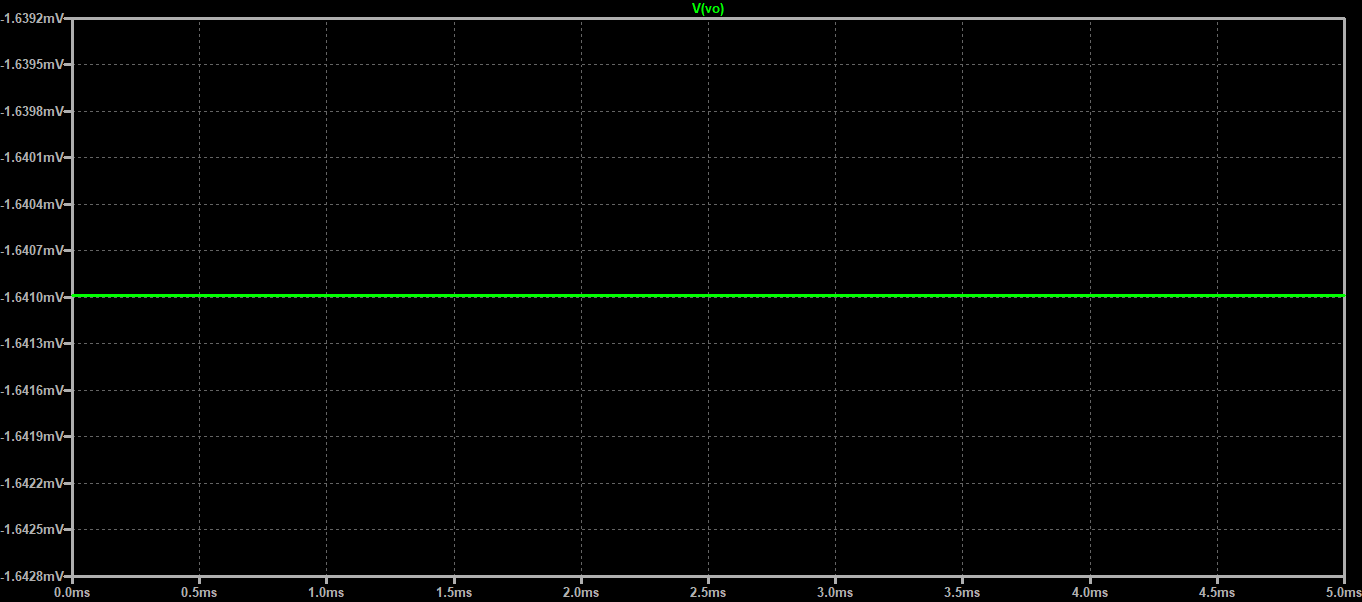
\includegraphics[scale=0.4]{Imagenes/Vo_Ios_CC.png}
    \caption{Vout(Ios)}
    \label{fig:enter-label}
\end{figure}
\begin{figure}[H]
    \centering
    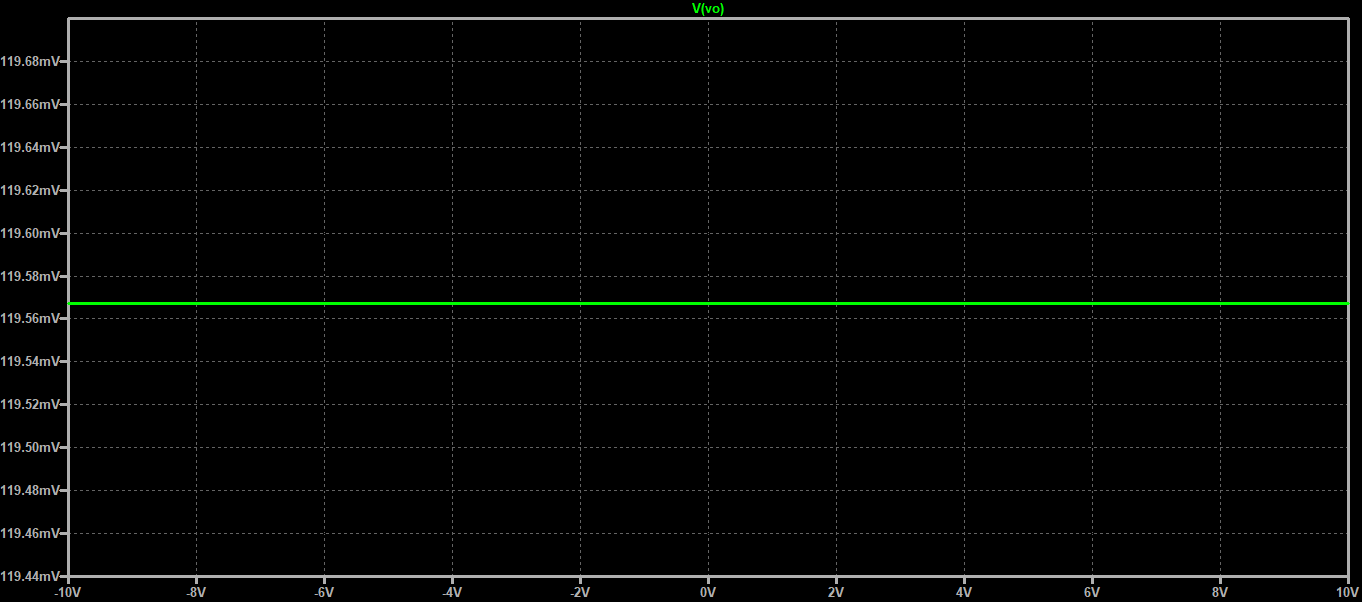
\includegraphics[scale=0.4]{Imagenes/Vo_Vos=2mV_CC.png}
    \caption{Vout(Vos)}
    \label{fig:enter-label}
\end{figure}
\newpage

\section{Caso de estudio para $R_i=100[k\Omega]$}
\subsection{Diseño de la etapa.}
Para este segundo caso, se deben cumplir los mismos requisitos del circuito anterior.
\paragraph{}
A partir de dichas especificaciones se obtiene:
\begin{equation}
    \nonumber
    R_i=50[\Omega] \longrightarrow Z_{i1,2} \geq 10R_i = 1[M\Omega]
\end{equation}
donde $Z_{i1,2} = R$.
\paragraph{}
Como el valor obtenido es el límite máximo admitido se toma $R=1[M\Omega]$. Si $A_{v1,2}(0)=30$
\begin{equation}
    \nonumber
    \frac{R_f}{R}=30 \longrightarrow R_f=30[M\Omega]
\end{equation}
\paragraph{}
En este caso $R_f >> 10[M\Omega]$ razón por la cual se hace uso de una red $T$ para cumplir con las especificaciones solicitadas.

\subsubsection{Red T.}
\onehalfspacing
Para el diseño de la \textit{red T} se debe tener en cuenta la relación entre $V_O$ y la corriente de alimentación $i_f$ que pasa por la resistencia $R_1$.
\paragraph{}
Suponiendo la entrada inversora a masa,
\begin{align}
    \nonumber
    i_f &= \frac{V_O}{R_2 + R_1||R_3}\cdot R_1||R_3 \cdot \frac{1}{R_1} \\
    \nonumber
    i_f &= \frac{R_3}{R_2\cdot R_1 + R_2\cdot R_3 + R_3\cdot R_1} \cdot V_O \\
    \nonumber
    \frac{V_O}{i_f} &= \frac{R_2 \cdot R_1}{R_3} + R_2 + R_1
\end{align}

\paragraph{}
Si $\frac{V_O}{i_f}=R_f$,
\begin{center}
    \boxed{R_f = \frac{R_2 \cdot R_1}{R_3} + R_2 + R_1}
\end{center}

\paragraph{}
Tomando  $R_1 = 100[k\Omega]$ y $R_2 = 220[k\Omega]$ con $R_f=30[M\Omega]$,
\begin{center}
    \boxed{R_3 = 741[\Omega]}
\end{center}

\paragraph{}
De esta manera se logran satisfacer todas las especificaciones.

\subsection{Cálculo de errores.}
\onehalfspacing
Con la incorporación de la red T la ganancia de lazo cambia a:
%\begin{equation}
%    \nonumber
%    T = - \frac{1}{2}\cdot \frac{A_d \cdot R \cdot R_3}{\left( 
%R_1 + \frac{R}{2} \right) \cdot \left( R_2 + R_3 \right) + R_2\cdot R_3}
%\end{equation}

\begin{equation}
    \nonumber
    T = - \frac{1}{2}\cdot \frac{A_d \cdot R \cdot R_3}{\left( 
R_1 + \frac{R}{2} \right) \cdot \left( R_2 + R_3 \right)}
\end{equation}

\subsubsection{Errores en DC.}
\onehalfspacing
\begin{equation}
    \nonumber
    \Delta V_{O}(v_{os}) = 2 \cdot \left( \frac{\left( 
R_1 + \frac{R}{2} \right) \cdot \left( R_2 + R_3 \right)}{R \cdot R_3} \right) \cdot v_{os} = 357,5v_{os} = 357,5\cdot 2[mV]  = 715[mV]
\end{equation}
\begin{equation}
    \nonumber
    \Delta V_{O}(I_{os}) = -R_f\cdot I_p^{-} = 30[M\Omega]\cdot I_p^{-} = 30[M\Omega]\cdot 45[\mu A]  = 1.350[V]
\end{equation}
\begin{equation}
    \nonumber
    \Delta V_{O}(A_d<\infty) = \frac{FS}{T_O} = \frac{10[V]}{280} = 35,7[mV]
\end{equation}
\begin{equation}
    \nonumber
    \Delta V_{O}(RRMC<\infty) = 0[V]
\end{equation}

\paragraph{}
El error total resulta: 

\begin{center}
    \boxed{\Delta V_{o} = 2,1[V]}
\end{center}

\subsubsection{Errores en AC.}
\onehalfspacing
\textbf{Ancho de banda de plena potencia.} 
\paragraph{}
\begin{equation}
    \nonumber
    f_{HP} = \frac{SR}{2\pi \cdot V_{pp}} =  \frac{0.5\left[ \frac{V}{uS} \right]}{2\pi \cdot 10[V]} = 8[kHz]
\end{equation}

\paragraph{}
\textbf{Ancho de banda de pequeña señal.} 
\paragraph{}
\begin{equation}
    \nonumber
    f_{HP} = k\cdot f_T = \frac{f_T}{A_{vfi}} = 33,3[kHz]
\end{equation}
Debido a que el amplificador utilizado en la simulación es de segundo órden, es decir tiene un polo que no permite que que el ancho de banda llegue a $1[MHz]$, sino que provoca la caída de $3dB$ en $2.7[kHz]$ es necesario recalcular para los $2.7[kHz]$:

\begin{equation}
    \centering
    \nonumber
    f_h = 0.9[kHz]
\end{equation}

\textbf{Error vectorial.} 
\paragraph{}
\begin{figure}[h!]
    \centering
    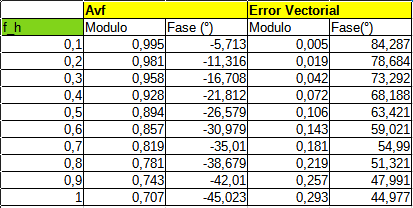
\includegraphics{Imagenes/tabla1.png}
    \caption{Error vectorial}
    \label{fig:enter-label}
\end{figure}
  
\subsection{Simulaciones.}
\onehalfspacing
A continuación se adjuntan las simulaciones para el circuito bajo estudio

\begin{figure}[h!]
    \centering
    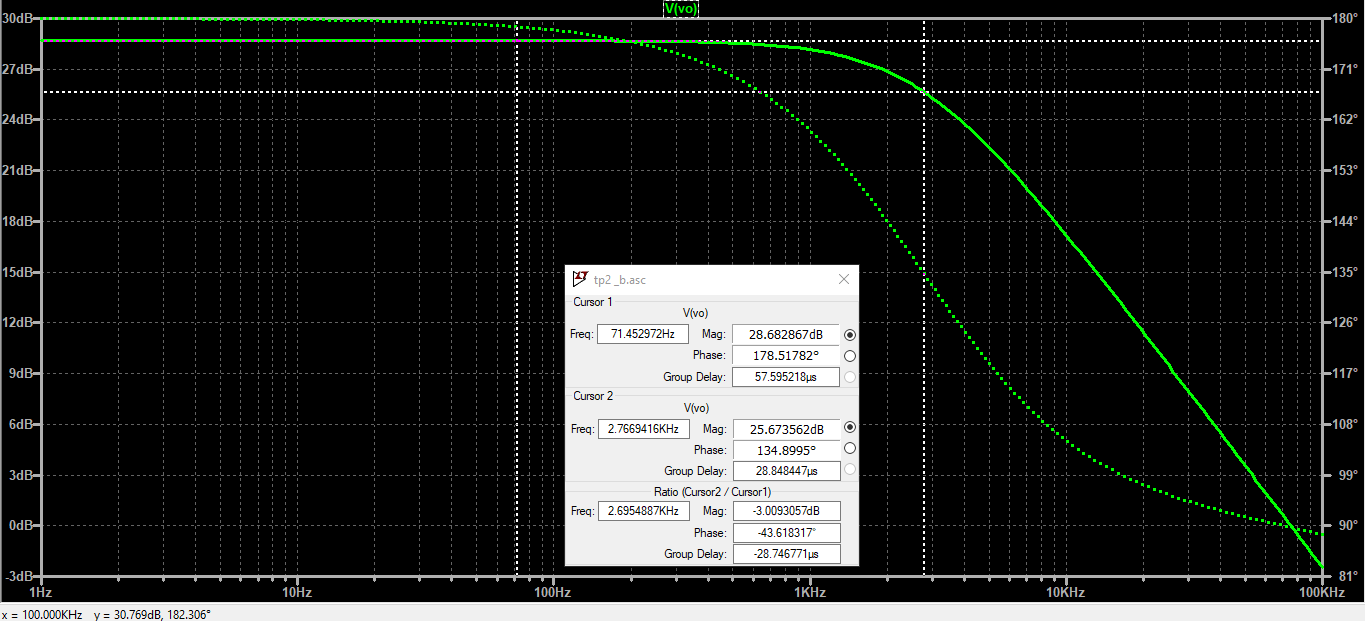
\includegraphics[scale=0.4]{Imagenes/bode_barrido2_hasta100k.png}
    \caption{Barrido en frecuencia, hasta $100kHz$}
    \label{fig:enter-label}
\end{figure}

\begin{figure}[h!]
    \centering
    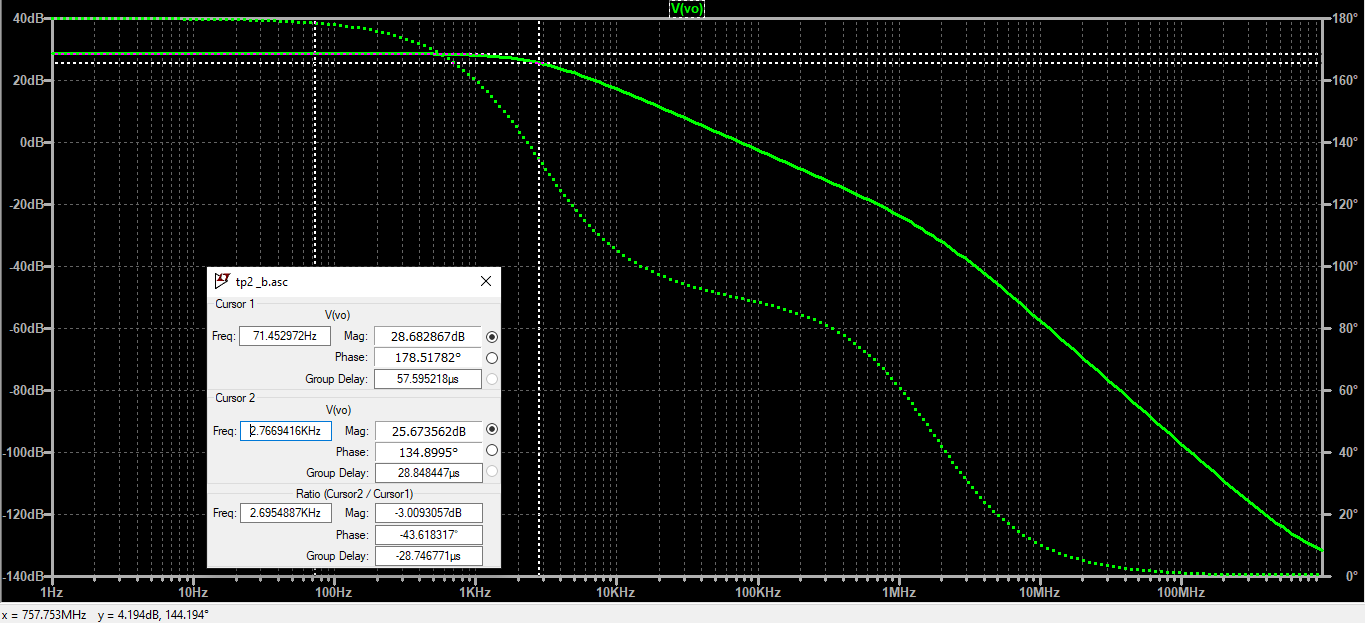
\includegraphics[scale=0.4]{Imagenes/bode_barrido2_hasta1G.png}
    \caption{Barrido en frecuencia, hasta $1GHz$}
    \label{fig:enter-label}
\end{figure}

\begin{figure}[h!]
    \centering
    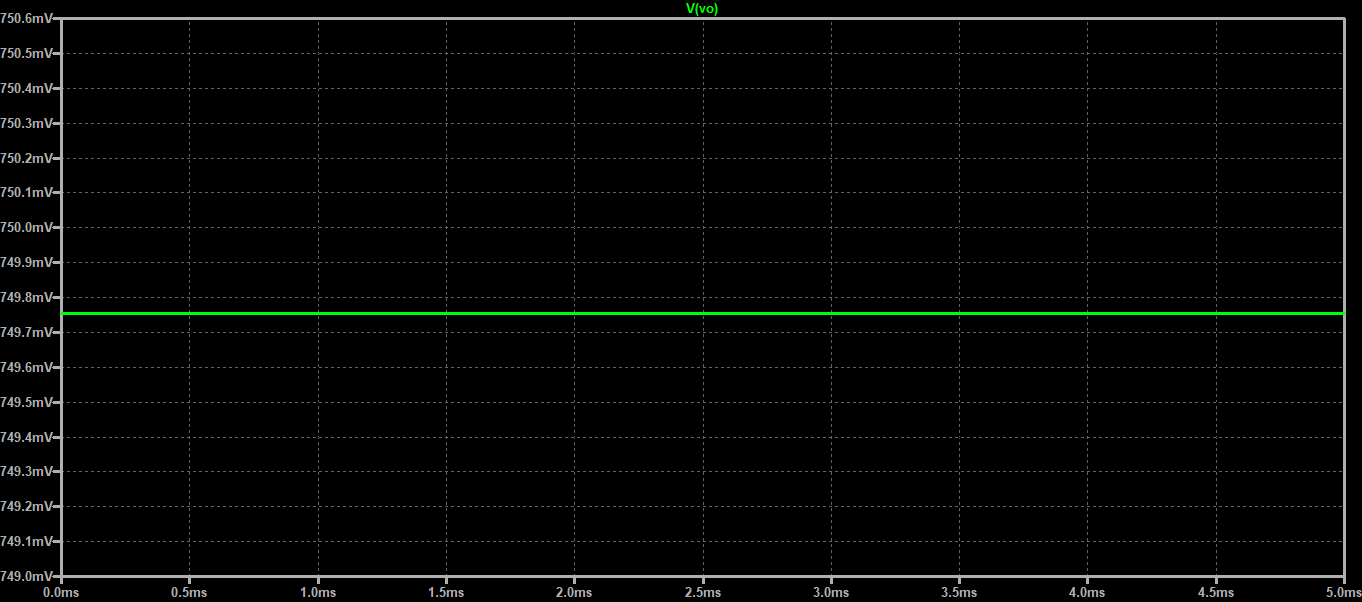
\includegraphics[scale=0.4]{Imagenes/2Vo_Ios_CC.png}
    \caption{Vout(Vos)}
    \label{fig:enter-label}
\end{figure}


\end{document}
